\documentclass[]{article}
\usepackage{lmodern}
\usepackage{amssymb,amsmath}
\usepackage{ifxetex,ifluatex}
\usepackage{fixltx2e} % provides \textsubscript
\ifnum 0\ifxetex 1\fi\ifluatex 1\fi=0 % if pdftex
  \usepackage[T1]{fontenc}
  \usepackage[utf8]{inputenc}
\else % if luatex or xelatex
  \ifxetex
    \usepackage{mathspec}
  \else
    \usepackage{fontspec}
  \fi
  \defaultfontfeatures{Ligatures=TeX,Scale=MatchLowercase}
\fi
% use upquote if available, for straight quotes in verbatim environments
\IfFileExists{upquote.sty}{\usepackage{upquote}}{}
% use microtype if available
\IfFileExists{microtype.sty}{%
\usepackage{microtype}
\UseMicrotypeSet[protrusion]{basicmath} % disable protrusion for tt fonts
}{}
\usepackage[margin=1in]{geometry}
\usepackage{hyperref}
\hypersetup{unicode=true,
            pdftitle={Offer Networks -- status update 2018/10},
            pdfborder={0 0 0},
            breaklinks=true}
\urlstyle{same}  % don't use monospace font for urls
\usepackage{graphicx,grffile}
\makeatletter
\def\maxwidth{\ifdim\Gin@nat@width>\linewidth\linewidth\else\Gin@nat@width\fi}
\def\maxheight{\ifdim\Gin@nat@height>\textheight\textheight\else\Gin@nat@height\fi}
\makeatother
% Scale images if necessary, so that they will not overflow the page
% margins by default, and it is still possible to overwrite the defaults
% using explicit options in \includegraphics[width, height, ...]{}
\setkeys{Gin}{width=\maxwidth,height=\maxheight,keepaspectratio}
\IfFileExists{parskip.sty}{%
\usepackage{parskip}
}{% else
\setlength{\parindent}{0pt}
\setlength{\parskip}{6pt plus 2pt minus 1pt}
}
\setlength{\emergencystretch}{3em}  % prevent overfull lines
\providecommand{\tightlist}{%
  \setlength{\itemsep}{0pt}\setlength{\parskip}{0pt}}
\setcounter{secnumdepth}{0}
% Redefines (sub)paragraphs to behave more like sections
\ifx\paragraph\undefined\else
\let\oldparagraph\paragraph
\renewcommand{\paragraph}[1]{\oldparagraph{#1}\mbox{}}
\fi
\ifx\subparagraph\undefined\else
\let\oldsubparagraph\subparagraph
\renewcommand{\subparagraph}[1]{\oldsubparagraph{#1}\mbox{}}
\fi

%%% Use protect on footnotes to avoid problems with footnotes in titles
\let\rmarkdownfootnote\footnote%
\def\footnote{\protect\rmarkdownfootnote}

%%% Change title format to be more compact
\usepackage{titling}

% Create subtitle command for use in maketitle
\newcommand{\subtitle}[1]{
  \posttitle{
    \begin{center}\large#1\end{center}
    }
}

\setlength{\droptitle}{-2em}

  \title{Offer Networks -- status update 2018/10}
    \pretitle{\vspace{\droptitle}\centering\huge}
  \posttitle{\par}
    \author{}
    \preauthor{}\postauthor{}
    \date{}
    \predate{}\postdate{}
  

\begin{document}
\maketitle

\hypertarget{what-is-offernets}{%
\subsection{What is OfferNets}\label{what-is-offernets}}

OfferNets is a research initiative\footnote{Based on previous and
  currently ongoing academic research: Weinbaum, D. (Weaver), \& Veitas,
  V. (2017). Open ended intelligence: the individuation of intelligent
  agents. Journal of Experimental \& Theoretical Artificial
  Intelligence, 29(2), 371--396.
  \url{https://doi.org/10.1080/0952813X.2016.1185748}; Veitas, V., \&
  Weinbaum, D. (2017). Living Cognitive Society: A `digital' World of
  Views. Technological Forecasting and Social Change, 114, 16--26.
  \url{https://doi.org/10.1016/j.techfore.2016.05.002}; Veitas, V.K.
  (2019). Synthetic Cognitive Development of decentralized
  self-organizing systems. PhD Thesis (forthcoming).} that aims at
creating a radically decentralized economy which is powered by diverse
network of independently operating and interacting agents. It combines
two R\&D paths which are tightly related yet embrace different levels of
abstraction:

\begin{enumerate}
\def\labelenumi{(\alph{enumi})}
\tightlist
\item
  \emph{Decentralized computing}: a massively scalable computing model
  and a software framework supporting asynchronous execution of
  heterogeneous processes concurrently using a shared data structure and
  allowing to model any mixture of emergent and controlled coordination
  among them.
\item
  \emph{OfferNets economy}: a decentralized economy providing
  alternative to purely currency based exchanges; it features a complex
  network of interactions and optimizes reciprocal exchanges of goods
  and services by finding agents with compatible and complementary
  preferences and coordinating their interactions.
\end{enumerate}

Research and development of (b) OfferNets economy is crucially dependent
on (a) Decentralized computing path but the importance and application
of the latter is much broader than the former. This means that we are
designing the decentralized computing and simulation modelling platform
to be maximally horizontally scalable beyond applications for OfferNets
economy.

\hypertarget{scope-directions}{%
\subsection{Scope \& directions}\label{scope-directions}}

\hypertarget{decentralized-computing}{%
\subsubsection{Decentralized computing}\label{decentralized-computing}}

The concept of open-ended decentralized computing\footnote{Based on
  previous and currently ongoing academic research: Weinbaum, D.
  (Weaver), \& Veitas, V. (2017). Open ended intelligence: the
  individuation of intelligent agents. Journal of Experimental \&
  Theoretical Artificial Intelligence, 29(2), 371--396.
  \url{https://doi.org/10.1080/0952813X.2016.1185748}; Veitas, V., \&
  Weinbaum, D. (2017). Living Cognitive Society: A `digital' World of
  Views. Technological Forecasting and Social Change, 114, 16--26.
  \url{https://doi.org/10.1016/j.techfore.2016.05.002}; Veitas, V.K.
  (2019). Synthetic Cognitive Development of decentralized
  self-organizing systems. PhD Thesis (forthcoming).} is an idea being
developed within OfferNets research initiative which allows
heterogeneous asynchronous processes to achieve spontaneous or guided
compatibility via indirect communication through a shared topological
space. The rationale of pursuing implementation and computational
testing of this model is to conceive a computational framework able to
perform large scale simulations of decentralized economy employing
different combinations of governance regimes and structures, multiple
currencies, barter networks and more. Furthermore, despite the model is
inherently decentralized, it allows to implement (or allow to emerge)
different levels of centralization as deem needed. The architecture of
the computational framework is documented in more detail
\href{https://singnet.github.io/offernet/public/offernet-documentation/conceptual-framework.html\#conceptual-architecture}{here}.

\hypertarget{simulation-engine}{%
\subsubsection{Simulation engine}\label{simulation-engine}}

The software architecture on which OfferNets simulations are run
consists of two large parts: (1) actor framework for powering
asynchronous execution of heterogeneous agents' logic and (2) graph
database powered by enterprise level graph database server for keeping
and updating the topology information on the network. For reading and
mutating topology information software agents we use Apache TinkerPop
graph computing engine.

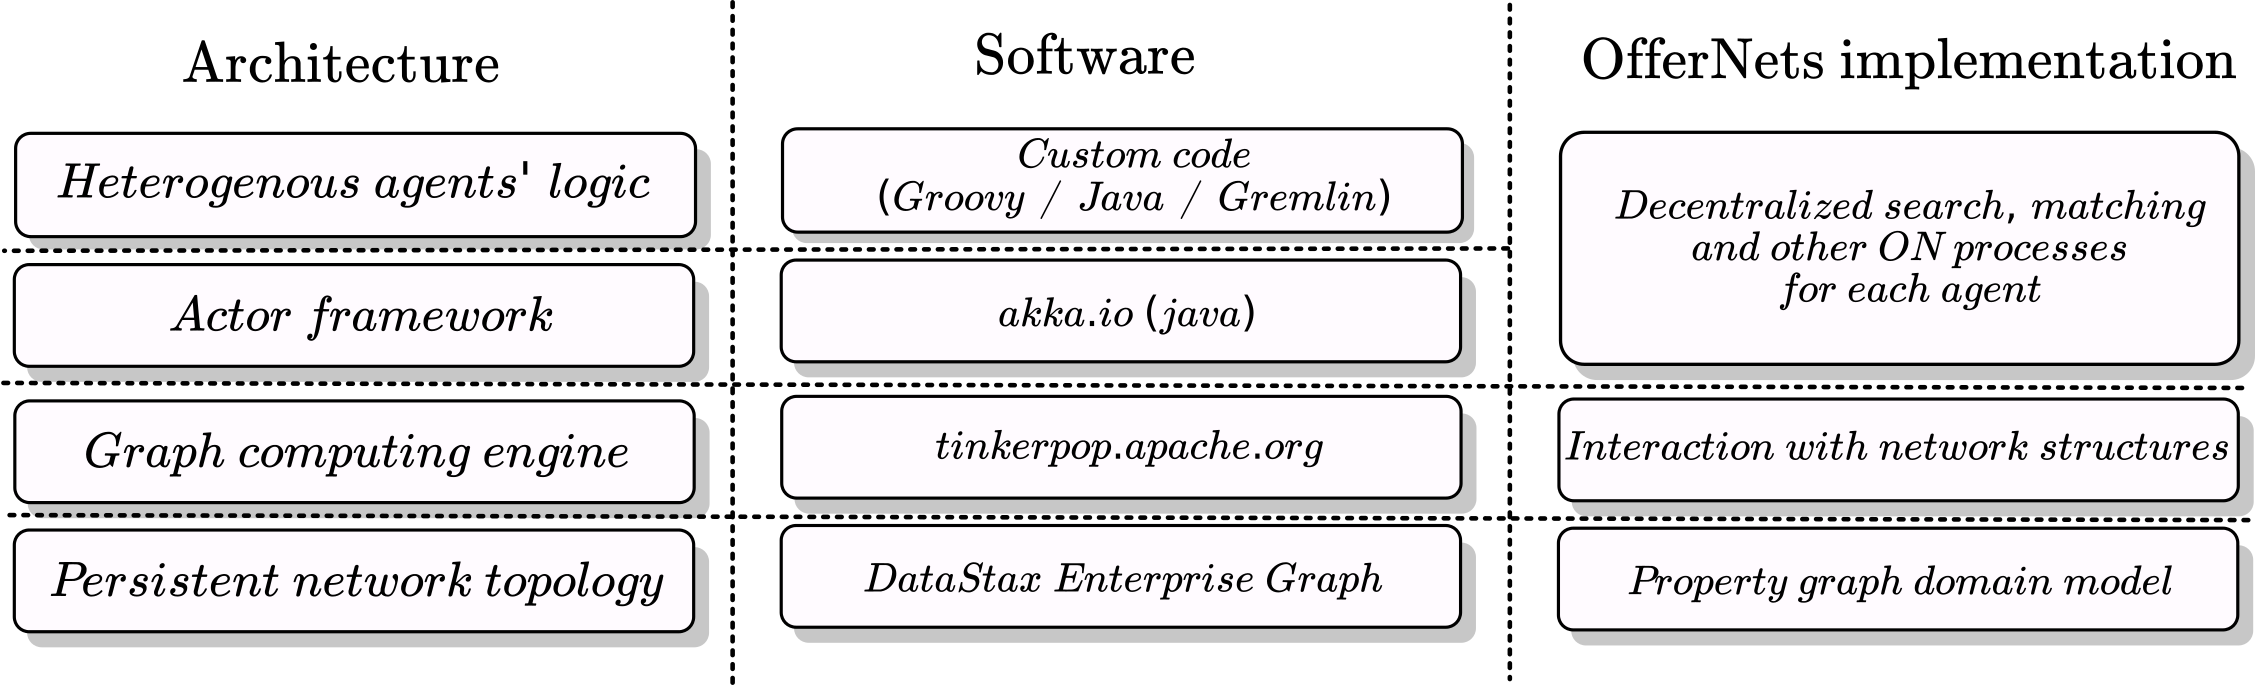
\includegraphics{pictures/stack.png}

\hypertarget{monitoring-and-analysis-engine}{%
\subsubsection{Monitoring and analysis
engine;}\label{monitoring-and-analysis-engine}}

\hypertarget{offernets-economy}{%
\subsubsection{OfferNets economy}\label{offernets-economy}}

\begin{itemize}
\tightlist
\item
  Specific OfferNets related computational aspects\footnote{Code is
    hosted at GitHub
    \url{https://github.com/singnet/offernet/tree/master/src/main/groovy};}
  (processes, etc.);
\item
  Simulation modelling: numbers of simulations, data points, etc.;
\item
  Documentation and electronic laboratory notebook;
\end{itemize}

\hypertarget{roadmap-and-status}{%
\subsection{Roadmap and status}\label{roadmap-and-status}}

\includegraphics{status_update-201810_files/figure-latex/timeline-1.pdf}

\hypertarget{integration-to-singularitynet-main-network}{%
\subsection{Integration to SingularityNET main
network}\label{integration-to-singularitynet-main-network}}

Conceptual aspects; technical aspects (massive simulations of the whole
network, reputation system, ai economy, decentralized self-organization
of different AI services);

\hypertarget{notes}{%
\subsection{Notes}\label{notes}}


\end{document}
